\chapter{Local DOB98 design, PI retuning, and attribution}
\label{ch:dob98}
The observer is identified around a physical speed of 9800 rpm; the number 98 does not describe model-fit accuracy. The independent multisine assesses the local predictor. The combined ramp/load cycle selects PI gains with the observer enabled and must be reported as selection evidence. The original-gain observer result is retained as a partial attribution check.

\section{A new inverse model at 9800 rpm and PI tuning after DOB engagement}
\textit{Archived October study. All simulations, searches, and checks described below predate this report.}\par

\subsection{Scope and identification experiment}
Previous PILCO is replaced in this comparison by DOB98 + tuned PI. Base PI, retuned Poly2 + PID and smooth PILCO retain their earlier gains and traces. The new controller uses no quadratic feedforward. Its structure is PI minus a filtered input-disturbance estimate, followed by the common fuel limits.

A new nominal model is identified specifically at 9800 rpm (98\% rated speed), with zero external shaft load. After preparation, training applies a deterministic binary fuel perturbation of amplitude 0.035 lbm/s, switched approximately every 0.18 s for 30 s. The base PI stabilizes the experiment; identification uses actual applied fuel, including the excitation, and actual shaft speed. Independent validation uses the sum of 0.37 and 1.17 Hz sinusoids, with amplitudes 0.025 and 0.015 lbm/s. No validation samples enter the least-squares fit.

Let $y_k=N_k-9800$ and $v_k=u_k-u_0$, with $u_0=2.530351198$ lbm/s and $T_s=0.015$ s. A parsimonious local model is
\begin{equation}y_{k+1}=a y_k+b v_k,\qquad
a=0.9789097769,\quad b=9.3039586704.\end{equation}
The parameters minimize the squared one-step residual over the excited training interval. The identified pole is stable, and the numerator has no finite nonminimum-phase zero. The model is local: the training speed varies only a few rpm around 9800. Independent free-run fit is 99.7829\%, with 0.001406 rpm RMSE. Fit means $100(1-\|y-\hat y\|/\|y-\bar y\|)$.
\par\noindent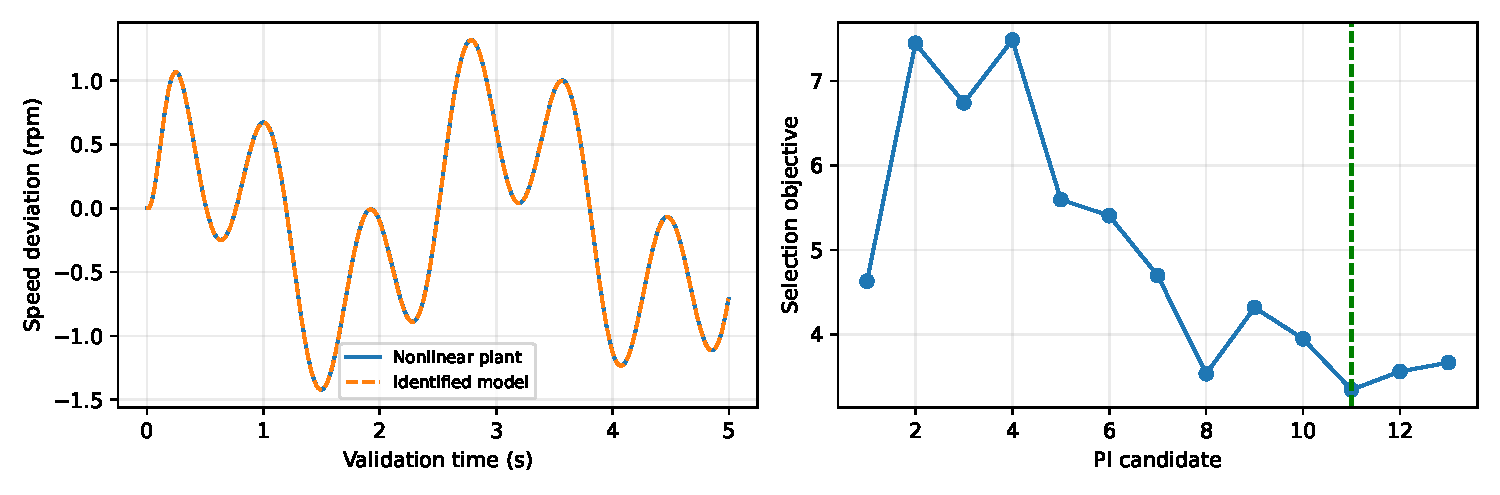
\includegraphics[width=\textwidth,height=.68\textheight,keepaspectratio]{late4_identification_tuning.pdf}
\subsection{Causal filtered inverse, step by step}
\textbf{1. Nominal speed dynamics.} With $q=z^{-1}$ denoting a one-sample delay,
\begin{equation}P_n(q)=\frac{bq}{1-aq}.\end{equation}
\textbf{2. Include the sensor.} Every controller retains the same physical sensor: time constant 0.05 s, unity gain, common initial conditions and noise disabled. The DOB uses its discrete approximation
\begin{equation}H_n(q)=\frac{(1-p)q}{1-pq},\qquad p=e^{-T_s/0.05}.\end{equation}
Thus the inverse is formed for sensed-speed dynamics $P_nH_n$. This approximation does not change the physical sensor blocks.

\textbf{3. Make the inverse causal and filtered.} Choose a unity-DC, two-pole low-pass filter with two delays:
\begin{equation}Q(q)=\frac{(1-r)^2q^2}{(1-rq)^2},\qquad r=e^{-2\pi f_cT_s},\quad f_c=1\ \mathrm{Hz}.\end{equation}
Then the two nominal delays cancel analytically:
\begin{equation}\frac{Q}{P_nH_n}=\frac{(1-r)^2(1-aq)(1-pq)}{b(1-p)(1-rq)^2}.\end{equation}
This is proper, causal and stable. A numerical frequency-response check verifies the identity, and an independent Python filter replay is compared with the recorded Simulink observer output.

\textbf{4. Estimate input-equivalent disturbance.} Use the known saturated command, without access to the external load signal:
\begin{equation}\hat d_{\rm raw}=\frac{Q}{P_nH_n}(N_s-N_0)-Q(u_{\rm cmd}-u_0).\end{equation}
The last estimate before absolute time 45 s is latched as a trim bias $d_0$. Compensation engages over the following two seconds, before the evaluation starts at 60 s:
\begin{equation}c=\operatorname{clip}\{0.7(\hat d_{\rm raw}-d_0),-1,1\},\qquad
u_{\rm cmd}=\operatorname{clip}\{u_{\rm PI}-c,0.2,4\}.\end{equation}
The compensation and fuel-command bounds are in lbm/s. The observer gain 0.7, cutoff 1 Hz and compensation limit 1 lbm/s are fixed engineering choices during the PI search; they are not claimed optimal.

\textbf{5. Tune PI after enabling the DOB.} The existing PI block uses $K_p(r-N_s)+K_i\int(r-N_s)dt$. Nine gain pairs, including the original (.025,.05), are followed by four local refinements. All candidates are evaluated with the DOB enabled on the requested combined cycle. Selection minimizes
\begin{equation}J=\mathrm{RMSE}_{0:25.005}+0.05R_{\rm seg},\end{equation}
where $R_{\rm seg}$ sums excess fuel total variation over 0--5, 5--10, 10--15 and 15--25.005 s. The weight is a numerical tuning weight with units rpm/(lbm/s). Invalid trajectories are rejected. This finite search selects $K_p=0.048$ and $K_i=0.05$; it does not establish a global optimum.
\subsection{Same combined cycle, revised four-controller comparison}
The target ramps from 9000 to 10000 rpm during relative seconds 0--5. A common 2789.650 hp external load is applied at second 10 and removed at second 15, followed by recovery through 25.005 s. The load is 10\% of the previously measured settled turbine power at 10000 rpm. Physical plant, sensor settings, reference, external load and fuel limits are matched. Saved comparator traces are reused because their implementations are unchanged.
\par\noindent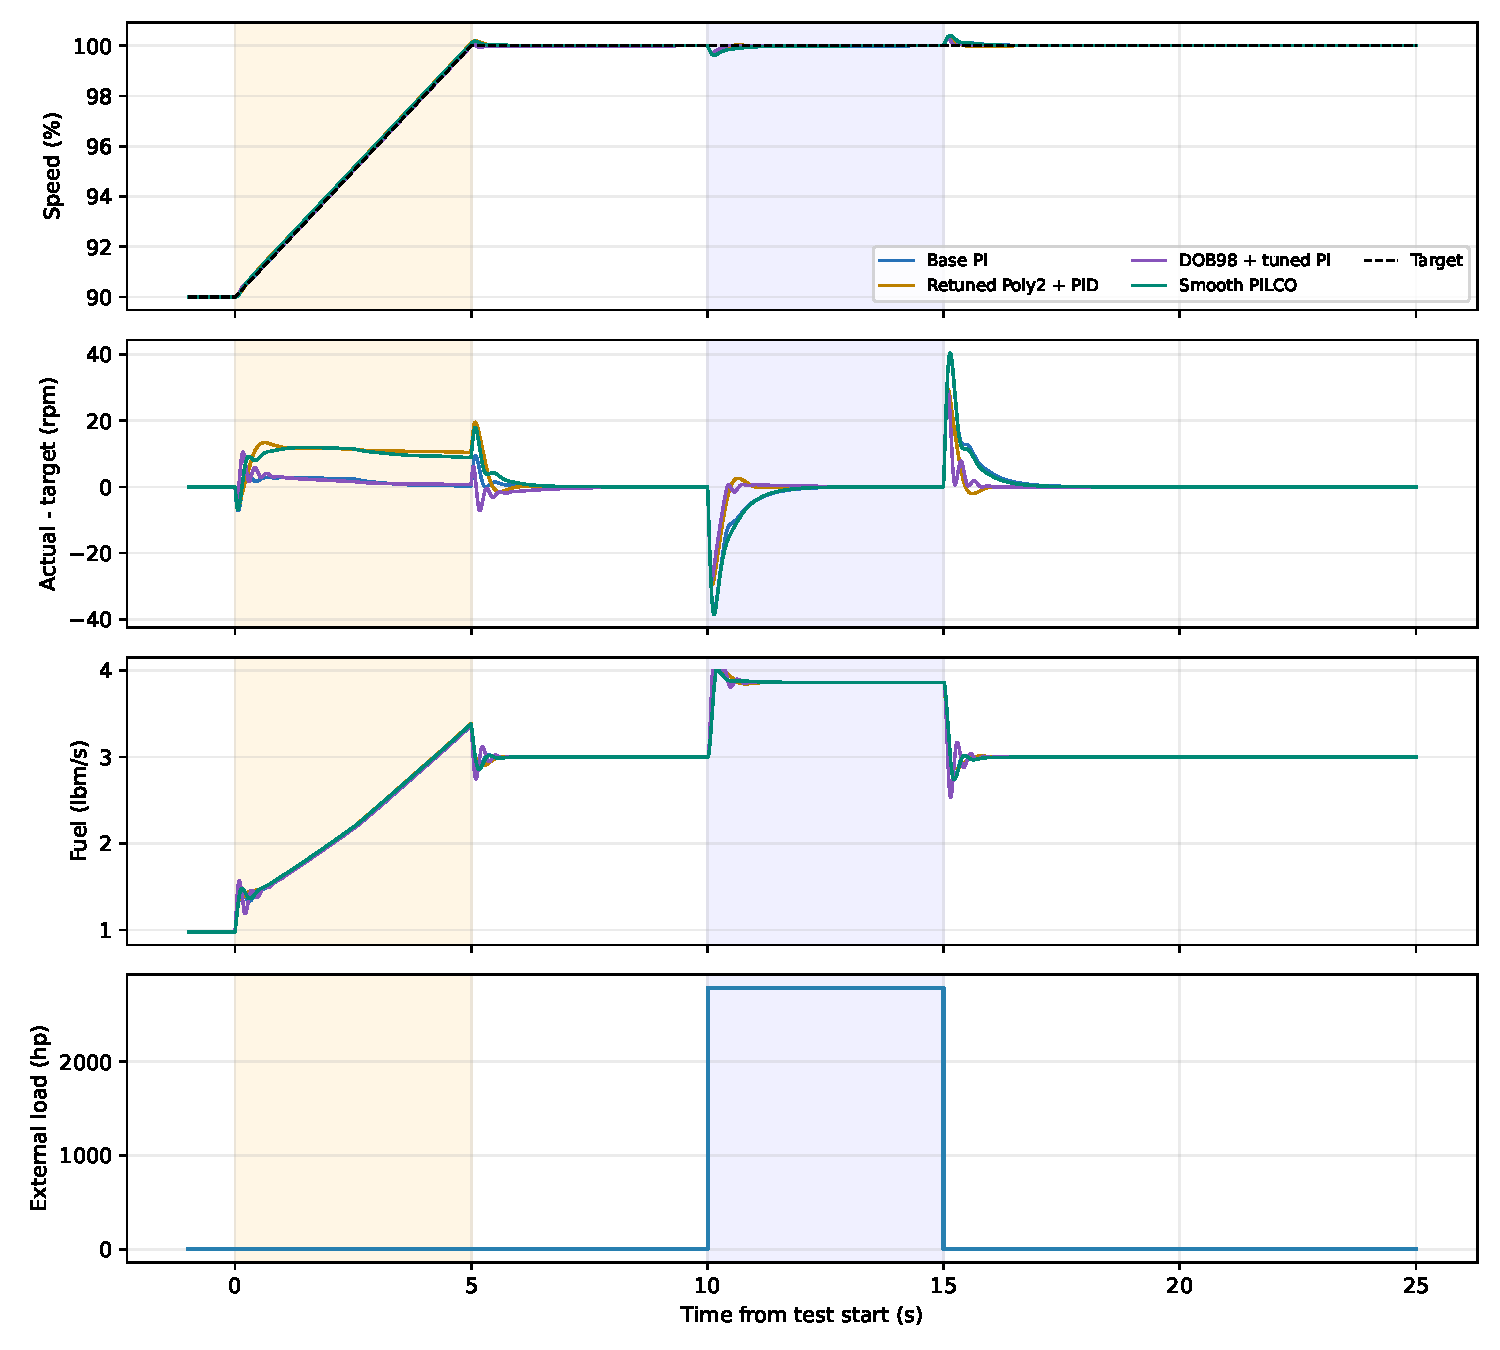
\includegraphics[width=\textwidth,height=.68\textheight,keepaspectratio]{late4_responses.pdf}
\subsection{Results and limits}
\begin{center}\small\begin{tabular}{lrrr}\toprule Controller & Ramp RMSE & Load/recovery RMSE & Full RMSE\\ & rpm & rpm & rpm\\\midrule
Base PI & 2.161 & 6.815 & 5.408 \\
Retuned Poly2 + PID & 10.949 & 4.416 & 6.214 \\
DOB98 + tuned PI & 2.459 & 3.710 & 3.142 \\
Smooth PILCO & 10.252 & 6.913 & 7.207 \\
\bottomrule\end{tabular}\end{center}
\begin{center}\small\begin{tabular}{lrrr}\toprule Controller & Load peak $|e|$ & Load excess TV & Min. surge\\ & rpm & lbm/s & \%\\\midrule
Base PI & 40.13 & 0.945 & 7.64 \\
Retuned Poly2 + PID & 29.39 & 0.696 & 7.75 \\
DOB98 + tuned PI & 29.10 & 2.184 & 7.74 \\
Smooth PILCO & 40.47 & 0.919 & 7.63 \\
\bottomrule\end{tabular}\end{center}
Errors use actual shaft speed, not sensed speed. Ramp RMSE covers 0--5 s; load/recovery RMSE covers 10--25.005 s; full RMSE covers the entire cycle. Load excess TV sums the 10--15 and 15--25.005 s segments. Sample interval is 0.015 s; first logged load-on is 10.005 s, and load-off is 15.000 s.

\textbf{Contribution of each change.} Base PI full-cycle RMSE is 5.408 rpm. Adding the DOB while retaining the original PI gains gives 4.546 rpm. Retuning PI with the DOB enabled gives 3.142 rpm. This ablation separates observer addition from gain tuning.

\textbf{Independent scenario check.} The selected gains are frozen and tested on a four-second speed ramp with a 5\% load pulse at seconds 10--15. Full-cycle RMSE is 2.024 rpm; minimum surge margin is 11.14\%. This check does not enter selection and is not a comparison against retuned baselines on that second scenario.

The requested combined cycle is a tuning case for DOB+PI, while the other gains were frozen from earlier studies. Consequently this is a comparison of the resulting controllers, not an equal-budget optimization contest. A local nominal model plus a DOB can tolerate some mismatch, but the small-excitation fit alone does not prove accuracy over 9000--10000 rpm. These nominal simulations are not a robust-stability proof. Fuel limits and compensation limits remain active parts of the implementation; the CSV records saturation and observer traces.
\subsection{Reproduction}
Run \path{dob98_identify_batch.m}, then \path{fit_dob98_model.py}, then \path{dob98_tune_batch.m}. The saved controller is \path{GasTurbine_DOB98_PI.mdl}, initialized by \path{tmats_dob98_setup.m}. Run \path{validate_dob98.py} for independent replay checks and \path{build_dob98_deliverables.py} for the revised figures and video. Data and selected parameters are under \path{results/dob98_pi_20261010}. Existing T-MATS workspace dependencies are required.


\section{Detailed interpretation of the final sensor and DOB results}
\subsection{Actual and sensed tracking answer different questions}
The sensor audit gives a particularly clear matched comparison because every maximum difference between the old and explicitly equalized trace is zero for actual speed, sensed speed, and fuel. The audit therefore rules out different sensor settings as the reason for the observed ordering. It does not imply that actual and sensed tracking errors are interchangeable.
\begin{table}[htbp]\centering\small
\begin{tabular}{lrr}\toprule Controller & Actual-speed ramp RMSE & Sensed-speed ramp RMSE\\ & rpm & rpm\\\midrule
Base PI & 2.160858 & 10.051133\\
Retuned Poly2 + PID & 10.948833 & 3.198864\\
Original PILCO-style PI & 11.223721 & 1.547154\\
Smooth PILCO & 10.251905 & 3.081877\\\bottomrule
\end{tabular}\caption{The same ramp scored using different signals. Values are from the archived sensor-comparison CSV; no new simulation is involved.}\end{table}
The original PILCO policy is closest to the target in sensed-speed RMSE and farthest in actual-speed RMSE among these four. A reader examining only the feedback error could therefore reach a different conclusion from the primary actual-speed comparison. For physical shaft regulation, the actual quantity is the relevant evaluation signal in this ideal simulation. In hardware it would need an independently justified measurement or state estimate.

\subsection{Deriving the local 9800-rpm identification explicitly}
Define $y_k=N_k-N_0$ and $v_k=u_k-u_0$. For each accepted identification transition, the equation $y_{k+1}=ay_k+bv_k+\epsilon_k$ supplies one row of the regression matrix:
\begin{equation}
\underbrace{\begin{bmatrix}y_1\\y_2\\\vdots\\y_M\end{bmatrix}}_{Y}
=\underbrace{\begin{bmatrix}y_0&v_0\\y_1&v_1\\\vdots&\vdots\\y_{M-1}&v_{M-1}\end{bmatrix}}_{X}
\underbrace{\begin{bmatrix}a\\b\end{bmatrix}}_{\theta}+\epsilon.
\end{equation}
Least squares chooses $\hat\theta$ to minimize $\|Y-X\theta\|^2$. The formula $(X^\top X)^{-1}X^\top Y$ explains the solution when full rank holds; numerically, a linear least-squares solver avoids unnecessary explicit inversion. The input must be the applied fuel including the excitation, because identifying against the injected perturbation alone would omit the stabilizing PI action.

One-step prediction uses the true $y_k$ in each row. Free-run prediction starts from an initial value and recursively uses $\hat y_k$. The archived model reports training one-step RMSE $1.7911\times10^{-4}$ rpm and free-run RMSE 0.003258 rpm. On the separate multisine record these are $9.8925\times10^{-5}$ and 0.001406 rpm. The small errors describe a speed range of only 9796.735--9803.056 rpm. A tiny local prediction error is entirely compatible with substantial mismatch at 9000 rpm or under a large external load.

\subsection{A directly implementable filtered inverse}
Write $r_f=e^{-2\pi f_cT_s}$ for the filter pole, to avoid confusing it with the speed reference, and define
\begin{equation}c_f=\frac{(1-r_f)^2}{b(1-p)},\quad
F(q)=\frac{Q}{P_nH}=c_f\frac{1-(a+p)q+apq^2}{1-2r_fq+r_f^2q^2}.
\end{equation}
If $w_k=N_{s,k}-N_0$ and $z=Fw$, then
\begin{equation}z_k=2r_fz_{k-1}-r_f^2z_{k-2}+c_f[w_k-(a+p)w_{k-1}+apw_{k-2}].
\end{equation}
The parallel filtered-command branch $h=Qv$ follows
\begin{equation}h_k=2r_fh_{k-1}-r_f^2h_{k-2}+(1-r_f)^2v_{k-2}.
\end{equation}
Thus the raw estimate is $z_k-h_k$. These recurrences explain why the two nominal delays are necessary in $Q$: the speed-inverse branch can be calculated from current and previous measurements, while the command branch explicitly retains the two delays. The construction uses the known saturated command; it does not read the external load schedule. Its poles are the filter poles, inside the unit circle, after the analytical cancellation specified by the model.

The trim latch subtracts the settled bias at handover. It removes a constant initial mismatch; it does not adapt the nominal model as speed changes. The compensation gain 0.7 and bound of 1 lbm/s are fixed during the PI search. The recorded maximum compensation in the selected main run is about 0.428413 lbm/s, below this compensation bound. The fuel command can nevertheless saturate because its total includes PI action as well as observer correction.

\subsection{What PI retuning bought and what it cost}
Adding the observer with the original gains reduces full-cycle RMSE from 5.407708 to 4.546279 rpm. Retuning to $(K_p,K_i)=(0.048,0.05)$ reduces it further to 3.142353 rpm. However, the original-gain DOB has ramp RMSE 1.441616 rpm, compared with 2.458988 rpm after retuning. The selected policy therefore trades some ramp performance for improved load/recovery behavior under the declared full-cycle objective.

The objective adds $0.05R_{\rm seg}$ to full RMSE. Its excess-variation windows include both the ramp and load phases. The load-only excess TV in the comparison table is a different subtotal. For the selected candidate these values are 4.085550 and 2.184455 lbm/s respectively. Confusing them would make the objective appear inconsistent with the displayed comparison. The selected controller also spends 1.139\% of full-cycle samples at a fuel limit, compared with 0.659\% for base PI. Better tracking is accompanied by additional actuator activity.

\subsection{The complete saved PI search}
\begin{table}[htbp]\centering\small\begin{tabular}{rrrrrrr}\toprule Case & $K_p$ & $K_i$ & Full RMSE & Ramp RMSE & $R_{\rm seg}$ & Objective\\\midrule
1 & 0.025 & 0.050 & 4.5463 & 1.4416 & 1.6970 & 4.6311\\
2 & 0.015 & 0.025 & 7.3993 & 7.9607 & 0.9555 & 7.4470\\
3 & 0.015 & 0.050 & 6.6614 & 2.0759 & 1.6012 & 6.7414\\
4 & 0.015 & 0.100 & 7.2924 & 5.7493 & 3.8650 & 7.4857\\
5 & 0.025 & 0.025 & 5.5285 & 6.6983 & 1.3702 & 5.5970\\
6 & 0.025 & 0.100 & 5.2704 & 5.4682 & 2.7144 & 5.4061\\
7 & 0.040 & 0.025 & 4.5578 & 5.3052 & 2.7683 & 4.6962\\
8 & 0.040 & 0.050 & 3.3854 & 2.0343 & 3.0062 & 3.5357\\
9 & 0.040 & 0.100 & 4.1326 & 5.5323 & 3.7298 & 4.3191\\
10 & 0.032 & 0.050 & 3.8400 & 1.6350 & 2.1835 & 3.9492\\
11 & 0.048 & 0.050 & 3.1424 & 2.4590 & 4.0855 & 3.3466\\
12 & 0.040 & 0.040 & 3.4183 & 1.7692 & 2.8927 & 3.5630\\
13 & 0.040 & 0.060 & 3.5107 & 2.9731 & 3.1287 & 3.6672\\
\bottomrule\end{tabular}\caption{All archived DOB98 PI candidates. RMSE is rpm; $R_{\rm seg}$ is lbm/s. Candidate 11 is selected by the stated objective.}\end{table}
Every candidate in the saved table is numerically accepted. This table describes a finite nine-pair search plus four refinements. It is not a proof that no untested pair could improve the objective, nor an equal tuning-budget comparison with the frozen Poly2 and PILCO methods. Candidate 1 is particularly useful because it isolates adding the DOB while retaining the original PI gains.

\subsection{The independent scenario and replay checks}
The frozen selected controller is then evaluated with a four-second 9000--10000 rpm ramp, corresponding to 250 rpm/s, and a 5\% load pulse. Its full RMSE is 2.024232 rpm, ramp RMSE 3.289699 rpm, and load/recovery RMSE 1.702970 rpm; minimum recorded surge margin is 11.135\%. The ramp metric uses the four-second interval, not the five-second interval of the tuning case. Other controller families were not retuned and compared on this independent scenario, so this result supports transfer of the selected controller but not a new ranking.

Independent filter replay matches the recorded observer branch within approximately $2.4\times10^{-13}$ lbm/s. The nominal filtered-inverse identity has maximum numerical error around $6.5\times10^{-14}$. These checks support correct coefficient ordering, delay handling, and filter realization. They do not establish uncertainty calibration, noise robustness, or a global stability margin for the nonlinear plant. Their proper role is to remove implementation ambiguity before interpreting the accepted plant trajectories.


